
\chapter{Design in reaction to CDCS}

From its very inception, Skedge's functionality and visual design were driven by the shortcomings of CDCS. Skedge is built \emph{bottom-up}, not \emph{top-down}---every aspect of the application was either made as a reaction to a particular grievance in CDCS or as the natural evolution of an existing feature. Skedge is thus rooted in \emph{usability} derived from real need, not mere conjecture along the question ``what could students want?''. Its success with students, shown in Chapter 4, demonstrates that this usability extends beyond my own standard and can fulfill the various discovered use-cases of students in general.

In this chapter, I invite the reader along on a tour of these grievances and their remedies.

%%%


\section{Modernity}

CDCS is an old system, relatively speaking, and its development on user-facing features has been almost entirely stagnant. It launched in 2009, seven years ago, and has hardly changed since. Figure \ref{fig:cdcs2010} shows CDCS in July 2010, which, besides the addition of a few search fields, is identical to its current version. Yet, since its introduction in 2009, we have seen the rise of mobile devices into ubiquity, a boom in ``hacker culture'' and public APIs, and the capability for standalone web applications to be as sophisticated and dynamic as desktop-class applications without the aid of browser extensions. With this in mind, Skedge brings course scheduling to the modern era.

\begin{figure}[ht]
  \centering
    \fbox{
      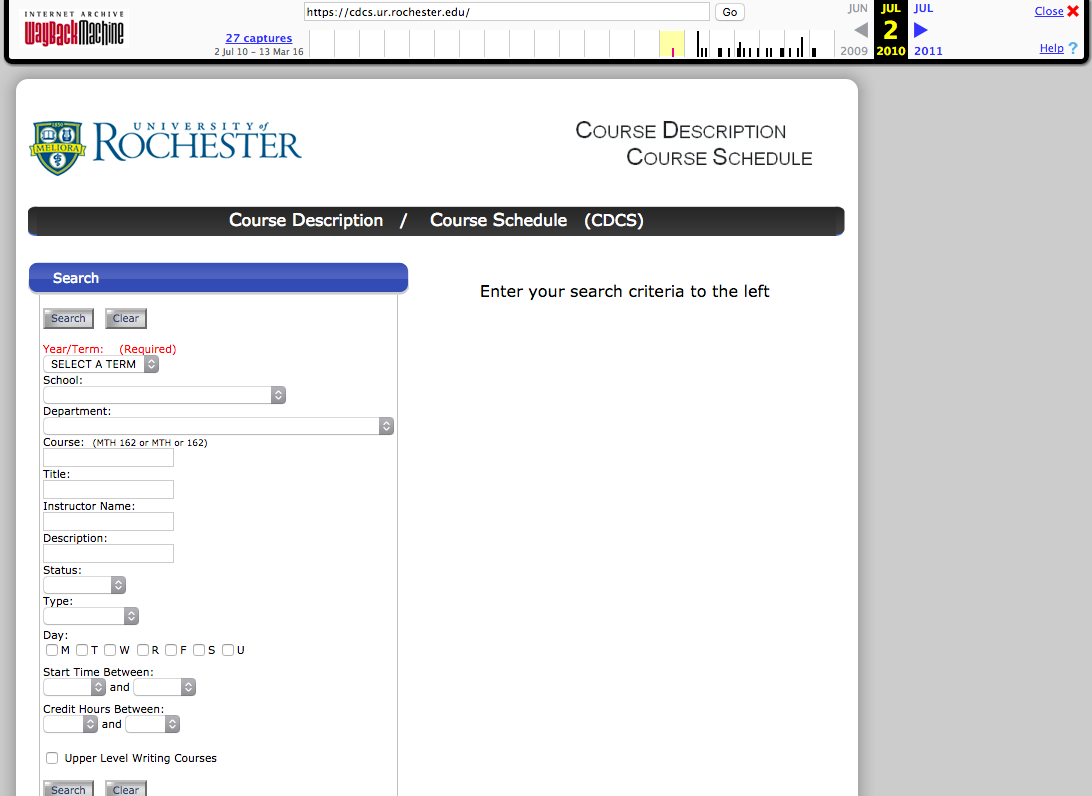
\includegraphics[width=10cm]{images/cdcs/2010}
    }
  \caption{CDCS in July 2, 2010, virtually unchanged from today, courtesy of \emph{Archive.org}}
  \label{fig:cdcs2010}
\end{figure}

\subsection{AJAX vs. GET requests}

CDCS makes an AJAX request with every submitted search, meaning that the server receives the request and returns a response all without any page navigation (i.e. the URL stays the same and no new page is loaded as the search results are displayed). Skedge, however, makes a GET request for every search submission, meaning that the user's browser loads a new page that contains the results and whose URL reflects the search query. This simple technical design decision substantially increases usability for two reasons:

\begin{enumerate}
  \item Page navigations allow users to leverage their browser history as it was designed---after making several searches, CDCS users who use the back button on their browsers will be brought to the page loaded before the very first use of CDCS, possibly losing time spent in crafting sophisticated searches. Skedge users can go backwards and forwards through their search histories and scroll locations using native browser functionality.
  \item Every search query has a unique URL (e.g. \url{http://skedgeur.com/?q=csc} for {\tt csc}), so users are able to send links to a specific course or search result to others. With CDCS, the URL remains \url{https://cdcs.ur.rochester.edu} throughout the duration of the session.
\end{enumerate}


\subsection{Mobile}

According to Mary Meeker's 2015 Mobile Technology Trends from Kleiner Perkins Caufield \& Byers\cite{kpcb}, in 2014, 51\% of adult time spent per day on the Internet was from a mobile device, versus 42\% spent on a desktop computer or laptop. Time spent on the Internet with mobile devices reached three hours per day in 2014, compared to less than one hour in 2010 (12\% mobile vs. 75\% desktop/laptop time share).

Undeniably, supporting mobile devices and tablets in web applications is crucial for usability nowadays. Note how Skedge is responsive to the user's device in Figure \ref{fig:sk-mobile}, compared with CDCS's lack of mobile support in Figure \ref{fig:cdcs-mobile}. CDCS on mobile requires the user to pinch and drag around both to read results and to make new searchs, while Skedge adapts content to the device's screen and fixes the search bar to the top of the screen for easy access while browsing.

Moreover, since no major mobile browser currently supports browser extensions (and if one did, the extensions themselves would most likely need to be re-architected), CDCS on a mobile device loses all scheduling functionality, unlike with Skedge on mobile.

\begin{figure}[ht]
  \centering
  \vspace{10pt}
  \begin{tabular}{c c}
    \begin{subfigure}[h]{4.5cm}
      \centering
      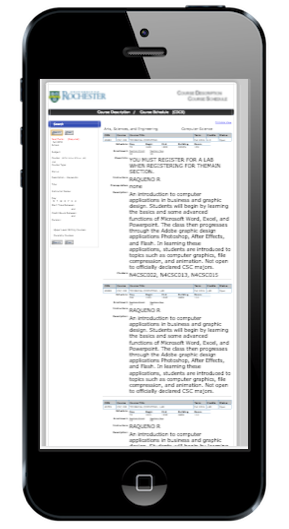
\includegraphics[width=1.00\textwidth]{images/cdcs/mobile}
      \caption{CDCS} \label{fig:cdcs-mobile}
    \end{subfigure}
    \begin{subfigure}[h]{4.4cm}
      \centering
      
\includegraphics[width=1.00\textwidth]{images/skedge/mobile}
      \caption{Skedge} \label{fig:sk-mobile}
    \end{subfigure}
  \end{tabular}
  \caption{CDCS and Skedge running on a mobile device}
\end{figure}

\subsection{Public API}

With the increasing number of attendees at University of Rochester's hackathons, it is clear that the University's ``hacker culture'' is growing---more students are collaborating to build side-projects that integrate resources and servies often benefitting the student community. Open-source and open-information services greatly help to foster such innovation, and having public APIs is essential toward this end.

Skedge provides a public JSON API at the root URL \url{http://www.skedgeur.com/api/}, made at the request of a student that was interested in using its course data, and the API has already been used in projects by several other student groups. The endpoints included are \url{/api/courses?q=query} (Skedge's query language---described in detail in section 2.3---is supported here), \url{/api/departments?q=optional_query}, and \url{/api/instructors?q=optional_query}.

\subsection{Built-in scheduler}

As explained in the introduction, Skedge offers users a course schedule right in the page, unlike CDCS which requires the Better CDCS browser extension for this functionality. Having a schedule native in the application has several advantages:

\begin{enumerate}
\item Besides some CDCS users possibly not even knowing about Better CDCS, not requiring a browser extension provides for a faster and more seamless user onboarding, especially when building schedules on public computers when extensions can't always be installed.

\item Skedge accommodates a schedule into its design, whereas Better CDCS has to work around an interface that wasn't designed with one. As a result, Better CDCS has lower usability, requiring the user to toggle between search results and their schedule. Skedge, conversely, gives users immediate visual feedback on how a course would fit into their schedule.

\item Schedule data is centralized on Skedge's servers as opposed to locally in a browser cache, meaning that it can synchronize across a user's devices or in sessions on public computers, persists browser resets, and can be easily publicly shared to other users.

\item Extensions like Better CDCS have limited browser support. Internet Explorer and mobile browsers are unsupported, for example.
\end{enumerate}

\clearpage

%%%


\section{Usability}

\subsection{Visual presentation}

Skedge offers several improvements over CDCS in the quality of its data presentation:

\begin{enumerate}
  \item Displaying information in a rigid, tabular way, CDCS does not leverage fonts and styling to adhere to typographical standards. Instead of using larger or bolder type, for instance, course titles are listed entirely in uppercase (e.g. ``INTRO TO PROGRAMMING''), which has been shown to be less readable than lower-case text \cite{caps}. This problem is compounded when users browse through possibly hundreds of courses. Skedge displays properly capitalized titles styled with large type that helps users to quickly group and locate them.

  \item While possibly not a fault of the CDCS system itself, there are very frequently typos or missing spaces in the ``comments'' section of courses, which Skedge corrects.

  \item CDCS displays all course times in 24-hour time, which, despite being concise and unambiguous, is not what most US students are used to. Skedge displays 12-hour time with AM/PM, and prevents ambiguities through the course-in-schedule visualization on hover.
\end{enumerate}

\subsection{Section display}

Often, courses are offered at multiple timeslots, sometimes taught by different instructors and in different rooms. These are called \emph{sections} of a course. CDCS displays each section in a discrete ``section box'' (all of which are nondistinct and have equal size), even if two sections pertain to the same course. (In this regard, CDCS should really be \emph{SDSS}, ``\emph{Section} Description / \emph{Section} Scheduler'', because it operates on the level of sections, not courses.) As a result, course descriptions (which can be lengthy), titles, prerequisites, comments, etc. are all repeated for every section of the course.

To make matters worse, many courses in the University course catalog include what I call \emph{subsections}---secondary sections associated with a course that must be registered for separately. Namely, these are labs, lab lectures, workshops, and recitations. Once again, CDCS displays \emph{all of these} as separate ``section boxes'' by default, and the course description is yet again repeated for each subsection (which, this time can be tens of times), wasting valuable page space.

Collapsing subsections within courses can result in massive improvements in filtering the data most relevant to the user. For instance, the search {\tt csc} for Fall 2016 on CDCS results in 147 ``section boxes'', while Skedge only shows 45 ``\emph{course} boxes'', with subsections collapsed within their respective course. This triage reduces the data (noise, more correctly) displayed by ~70\%, and is even higher for departments with more abundant labs and workshops, such as Physics (Skedge: 35 vs. CDCS: 226, an ~85\% reduction), or Chemistry (Skedge: 25 vs. CDCS: 171, an ~86\% reduction).

Skedge can reduce the amount of data to scroll through---and thus the time taken to do so---by six- or seven-fold (and possibly more, counting the attention users otherwise have to pay to distinguish course from subsections), so this design decision has a large usability payoff.

Additionally, some Physics courses (for instance) follow the ``A / B'' subsection structure, where a student registered for an ``A Section'' (as opposed to the ``B Section'') must also register for an ``A Lab'' and ``A Workshop''. Skedge organizes subsections for these cases to help sort the two out, which get mixed up in CDCS's linear output.

Note that in Figure \ref{fig:cdcs-sections} (CDCS), the first two boxes are sections for the same course, and the next two are labs for that course. Four more lab sections and \emph{twenty} more workshop sessions for that same course follow below the truncated screenshot. Figure \ref{fig:sk-sections} (Skedge) demonstrates how this information can be conveyed more concisely.

\begin{figure}[ht]
  \centering
  \vspace{10pt}
  \begin{tabular}{c c}
    \begin{subfigure}[h]{6cm}
      \centering
      \fbox{
        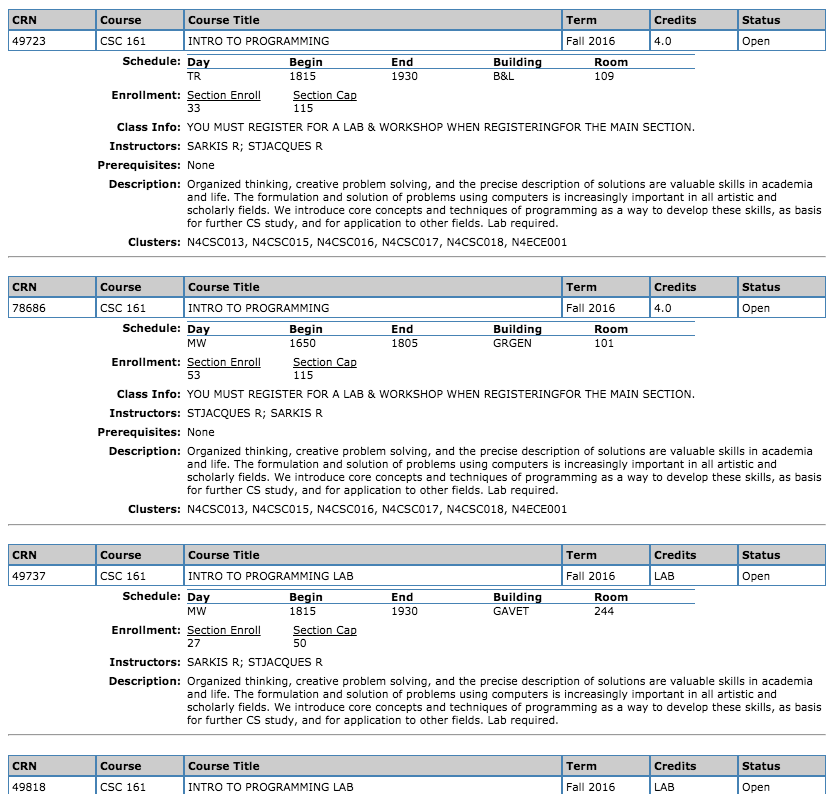
\includegraphics[width=1.00\textwidth]{images/cdcs/sections}
      }
      \caption{Ungrouped sections in CDCS} \label{fig:cdcs-sections}
    \end{subfigure}
    \hspace{15pt}
    \begin{subfigure}[h]{7cm}
      \centering
      \fbox{
        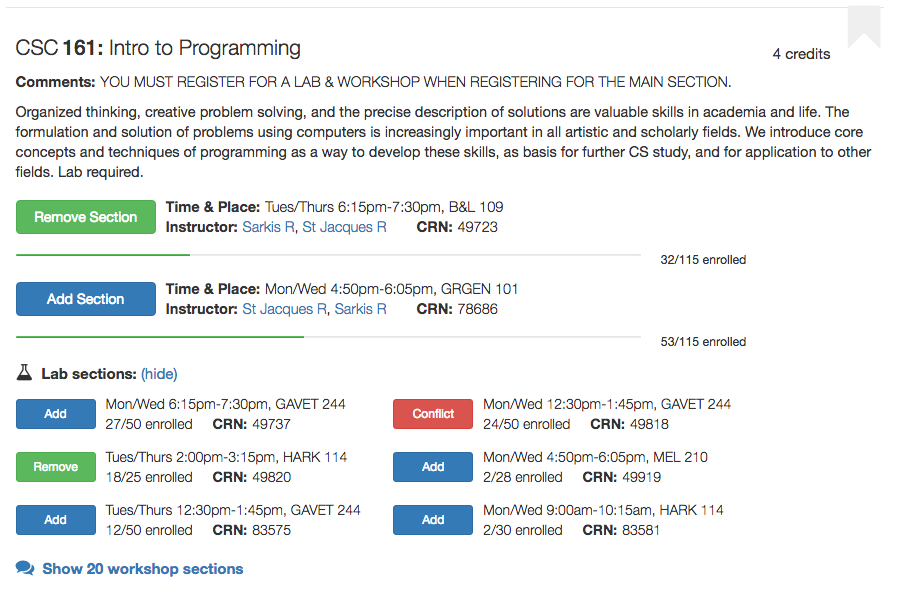
\includegraphics[width=1.00\textwidth]{images/skedge/sections}
      }
      \caption{Grouped sections in Skedge} \label{fig:sk-sections}
    \end{subfigure}
  \end{tabular}
  \caption{Section and subsection presentation in CDCS and Skedge}
\end{figure}


\subsection{Course reference}

\emph{Course mentions} will often appear in the prequisites, crosslists, comments, or description fields of a course (e.g. ``\textbf{Prerequisites:} CSC 171 or equivalent; MTH 150 is REQUIRED''). Users frequently want to find out more information about mentioned courses (frequency shown in Chapter 4). In CDCS, because course mentions are displayed as ordinary plaintext, users have to scroll back up, make a search for \emph{that} course, and lose their current search context as a result.

Skedge solves this by linking each course mention to its search query, in the style of Wikipedia. Moreover, it prevents context-switches by displaying a popover containing information on that course when the user hovers their cursor over the course mention (see Figure \ref{fig:sk-hover}).

\begin{figure}[ht]
  \centering
  \vspace{2pt}
  \fbox{
    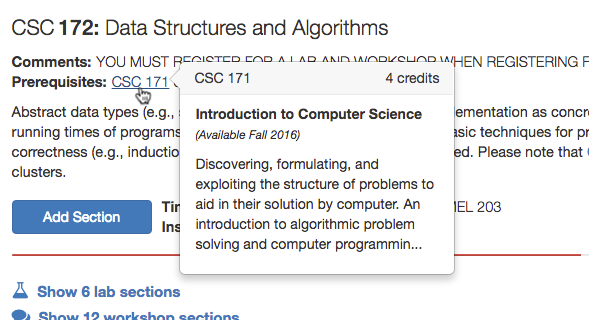
\includegraphics[width=8cm]{images/skedge/hover}
  }
  \caption{Hoverable and clickable course mention in the \emph{Prerequisites} field of a course} \label{fig:sk-hover}
\end{figure}

\subsection{Multiple schedule support}

With an active schedule still in use, students often want to plan their next semester's schedule. This is impossible with the Better CDCS extension, which instead adds courses from both terms to the same schedule, sometimes causing non-existent conflicts. A CDCS user must clear their entire schedule out before scheduling a new one. On Skedge, however, when a user adds a section of a term for which they do not yet have a schedule, a new one will automatically be created for that term. Users are also able to access their old schedules.

Additionally, a common feature request for Skedge is the implementation of multiple schedules \emph{per} term, allowing users to experiment with different schedule possibilities.\footnote{Currently under development, but simple to implement given the existing schedule management structure.}

\clearpage

%%%


\section{Search friendliness}

Of course, the most important usability concern for a course explorer/scheduler is being able to effectively \emph{find courses}.

In this section, I will present the \emph{Skedge DSQL}, a domain-specific query language that is based on natural language. Next, I will demonstrate how Skedge leverages the DSQL to handle the three search criteria students have for finding courses better than CDCS does.

\subsection{Natural language search}

In the spirit of this chapter's theme, Skedge's search method was, again, primarily designed as a reaction to CDCS's. CDCS's search method is a 15-field form (see Figure \ref{fig:cdcs-search}), of which I only found myself regularly using two (one of them being the \emph{required} ``Year/Term'' field). This prompted me to closely examine the fields to a) determine redundancies between them and b) find how to make some of the valuable filter fields more usable. From this came Skedge's unified, natural language based search method, which I call the \emph{Skedge Domain-Specific Query Language (Skedge DSQL)}. Figure \ref{fig:sk-search} is a list of example possible searches shown to users as they type.

\begin{figure}[ht]
  \centering
  \vspace{5pt}
  \begin{tabular}{c c}
    \begin{subfigure}[w]{4.5cm}
      \centering
      \fbox{
        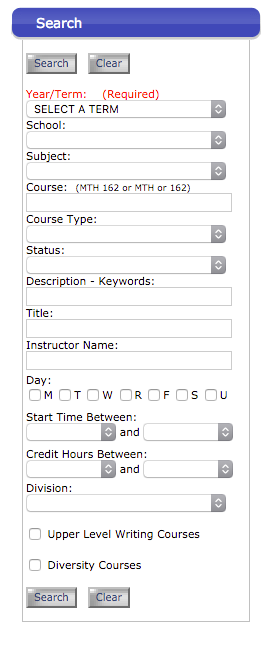
\includegraphics[width=3.3cm]{images/cdcs/search}
      }
      \caption{Form-based search in CDCS} \label{fig:cdcs-search}
    \end{subfigure}
    \hspace{5pt}
    \begin{subfigure}[w]{8.5cm}
      \centering
      \fbox{
        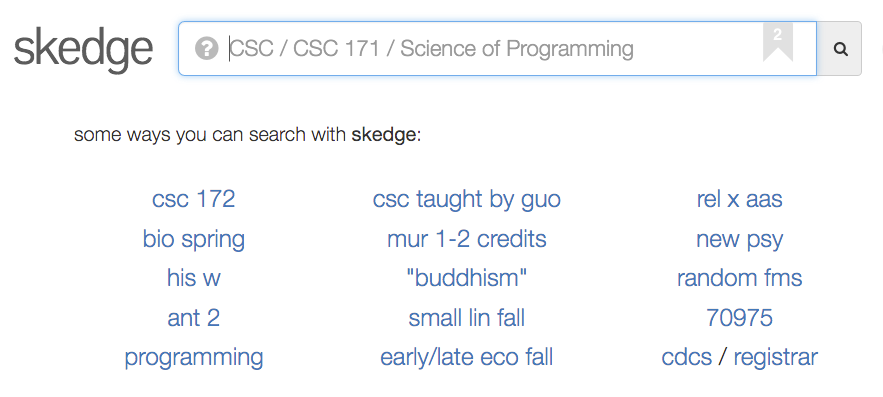
\includegraphics[width=1.00\textwidth]{images/skedge/search}
      }
      \caption{Examples of the Skedge DSQL} \label{fig:sk-search}
    \end{subfigure}
  \end{tabular}
  \caption{Two philosophies of search method}
\end{figure}

\begin{figure}[ht]
  \centering
  \vspace{10pt}
  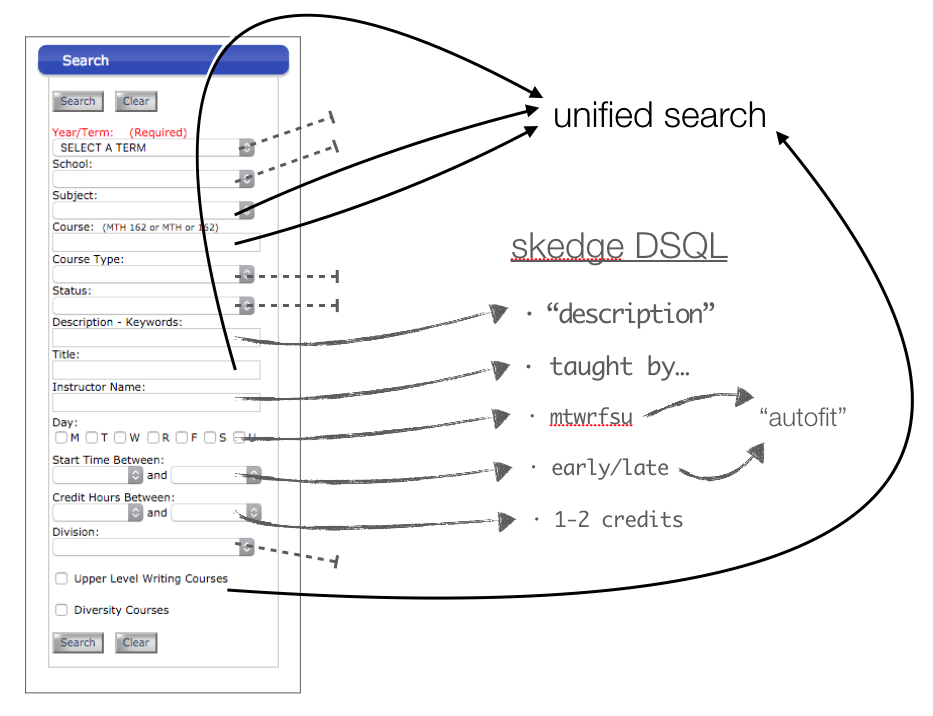
\includegraphics[width=14cm]{images/search-mapping}
  \caption{Mapping from CDCS's form-based search to the Skedge DSQL} \label{fig:search-mapping}
\end{figure}

Figure \ref{fig:search-mapping} is a mapping of each CDCS field to an element of the Skedge DSQL or unified search. Dashed lines that end abruptly are fields that were deemed unnecessary or redundant due to a Skedge-unique feature. To briefly sum up my rationale for each field:

\onehalfspacing

\subsubsection{Removed fields}

\begin{enumerate}

  \item \emph{School} (e.g. ``College of Arts, Sciences, \& Engineering'', ``Eastman School of Music'', etc.) was removed in favor of always searching all schools, as is the default on CDCS. Searching by department codes (which are unique across schools) designates a school regardless.

  \item \emph{Course Type} (e.g. ``Main Course'', ``Lab'', ``Workshop'' etc.) was removed because Skedge already embeds subsections into courses.

  \item \emph{Status} (i.e. ``Open'', ``Closed'', or ``Cancelled'') was removed because it is often useful to see closed courses if there is possibility of the instructor letting in more students, and searching for cancelled courses did not seem useful.

  \item \emph{Division} (i.e. ``Humanities'', ``Social Sciences'', etc.) was removed because it seems too broad to be useful, but it could be added to the Skedge DSQL if there is demand.

\end{enumerate}

\subsubsection{Unified Search (left side)}

The \emph{unified search} components can be entered directly into the single Skedge search field, along with the Skedge DSQL. It includes the CDCS fields:

\begin{enumerate}
  \item \emph{Subject} (department).
  \item \emph{Course} (department code and/or course number, e.g. ``csc 171'').
  \item \emph{Title} (course title).
\end{enumerate}

\subsubsection{Skedge DSQL (right side)}

The \emph{Skedge DSQL} is enterable using special keywords and, optionally, qualifiers for those keywords. It includes the CDCS fields:

\begin{enumerate}
  \item \emph{Year/term}, which is no longer required. It maps to the keywords {\tt \{spring,fall,summer,winter\}} and a four-digit year to specify term and year, and defaults to the current year and term.

  \item \emph{Description}, which is specified by surrounding the query in quotes (e.g. ````buddhism'''').

  \item \emph{Instructor name}, which is specified with the keyword {\tt taught by} and given the instructor name as a qualifier (e.g. ``taught by Guo'').

  \item \emph{Day}, which can be specified with the keywords {\tt \{m,t,w,r,f,s,u\}} for filtering by specific days of the week (e.g. ``mwf'' for Monday-Wednesday-Friday classes only).

  \item \emph{Start time between} is replaced by the keywords {\tt \{early,late\}} which \emph{sort} (ascending and descending, respectively) the results by start time.

  \item \emph{Credit hours between} is replaced by the keyword {\tt credits}, qualified with a number or range (e.g. ``dan 1-2 credits'' for Dance classes with 1-2 credits).

  \item \emph{Upper level writing} is replaced by the single-letter keyword {\tt w} (e.g. ``his w'' for History upper-level writing courses).
\end{enumerate}

\doublespacing

As noted in Figure \ref{fig:search-mapping}, many use-cases for the \emph{Day} and \emph{Start time between} fields can be obsoleted with an \emph{autofit} feature that will be described later in the next subsection.

  \subsubsection{Advantages of the DSQL}

    The main advantage of Skedge's search system is in its reduction of 15 fields to a single one. I hypothesize that since the vast majority of searches fit the department code / course number pattern (this hypothesis later supported in Chapter 4), the time required to force the user to select a term and then find the correct box to enter this query is wasted.

    In addition, once learned and remembered, using a natural language based query language can be faster and more intuitive than clicking on form fields. And more importantly, the Skedge DSQL is more easily extendable as new search features are invented. For CDCS, the more form fields that are added to the sidebar, the less usable its user interface becomes. For Skedge, while it may take longer for users to learn a bigger DSQL, there is no issue with crowding user interface real estate.
  
  \subsubsection{Disadvantages of the DSQL}

    One disadvantage of Skedge's DSQL is the possible grammatical ambiguity of some queries. For instance, the query ``Fall of the Roman Empire'' could be searching for courses with that as the title, or searching for courses in the \emph{fall term} with the title ``of the Roman Empire''. Unless multiple queries are run and more complex natural language processing is done, the system would have a hard time disambiguating between the two. This could also be solved with a ``did you mean?'' feature, which disambiguates a query into every possible DSQL breakup.
    
    Another notable disadvantage of the DSQL is having to know it, and it having a possibly steep learning curve for some users. However, the argument will be made in Chapter 4 that simply by using the site over time, users will self-learn the Skedge DSQL. One of the ways this is possible is thanks to Skedge's search system being \emph{multi-purposed}. Hyperlinks around the site---instructor names (which link to ``{\tt taught by <name>}''), course references, or schedule course blocks for example---all direct the user to an ordinary search results page with the search field populated, signalling to the user that such a search is possible.


\subsection{Course selection criteria}

I have identified \emph{three} use-cases for course searching (the existence of and distinction between these cases will be demonstrated with collected usage data in Chapter 4). The three cases are \textbf{requirements}, \textbf{electives}, and \textbf{peer recommendations}. The Skedge DSL and other application features offer substantial improvements over CDCS for each of these cases. 

  \subsubsection{Requirements}

  These are courses that are required for a student to complete their degree, and are typically searched for directly. The functionality required here is simple and is mostly satisfied by CDCS, but Skedge offers the following improvements to the process:

  \begin{enumerate}
    \item \emph{Crosslisted courses:} For students with more than one major and/or minor, searching for courses that are crosslisted between departments can be valuable in reducing their requirement load. This search filter is unsupported by CDCS, and is supported by Skedge using the operator ``{\tt x}'' (e.g. ``{\tt csc x ece}'' for courses listed under both Computer Science and Electrical \& Computer Engineering departments).

    \item \emph{Clusters:} Skedge already stores a users' previously taken courses, so it can intelligently suggest either already-completed clusters or courses that would complete clusters that are missing one or two courses. For students with many degree requirements already, this could greatly reduce time spent navigating the University's Cluster Search Engine (for which I also have a long list of grievances, but that lies outside the scope of this paper.)\footnote{This feature is under development and is not currently live. It was, incidentally, requested by a Skedge user.}

    \item \emph{CRN:} Surprisingly, search by Course Reference Number is unsupported by CDCS. It is supported by Skedge by just searching the 5-digit number.
  \end{enumerate}

  \subsubsection{Electives}

  Elective courses can either be courses that are required for a major or minor, but are chosen by the student, or they can be courses of particular interest to students who have the flexibility to take them. For this use-case, Skedge offers search, filter, and sorting features that substantially aid users in browsing through courses and discovering ones they might want to take. Note that none of the following features are supported by CDCS.

  \begin{enumerate}

    \item The Skedge DSQL includes the ``new'' keyword, which qualifies an accompanying search by only displaying the courses that were not offered the previous year for that term. For instance, searching ``new csc'' today (Fall 2016) would show Fall Computer Science courses that have been added to the catalog or changed since Fall 2015.
    \item The Skedge DSQL could include an ``autofit'' keyword, which would take into account the user's current schedule, and only show sections that would not conflict with any already scheduled times.\footnote{This feature is under development and is not currently live.}
    \item The Skedge DSQL includes the ``random'' keyword, which displays a single random course matching the accompanying query. For instance, ``random csc'' would show a random course in Computer Science for the current term. Used in conjunction with ``autofit'', it can a powerful way to find interesting new classes that are available for users to try.
    \item The Skedge DSQL includes sorting by class size---useful for students trying to find smaller, discussion based classes---or by class starting time---for students with preferences of morning or afternoon/evening classes.
    \item Instructor names appearing in courses automatically link to searches for more courses taught by that instructor, which is easier than having to use the CDCS ``instructor'' field to make a separate search.

  \end{enumerate}

  \subsubsection{Peer Recommendations}

  CDCS currently has no support at all for peer course recommendation, a highly undervalued resource for course finding. Skedge implements peer recomendations through Skedge Social, a system detailed in the next section.
  
\clearpage

%%%


\section{Peer connectivity}

The question ``what are you taking this semester?'' may possibly be the most common phrase uttered in campus smalltalk within the first few weeks of a semester. But students' social lives do not solely exist in-person---social media dominates college social lives etc, v impt to consider [CITE]. The ``what are you taking'' question typically translates to social media in the form of the schedule image exported from Better CDCS posted to Facebook (e.g. Figure \ref{fig:cdcs-social}). There are several limitations to this model.

\begin{figure}[H]
  \centering
  \vspace{5pt}
  \begin{tabular}{c c}

    \begin{subfigure}[w]{7cm}
      \centering
      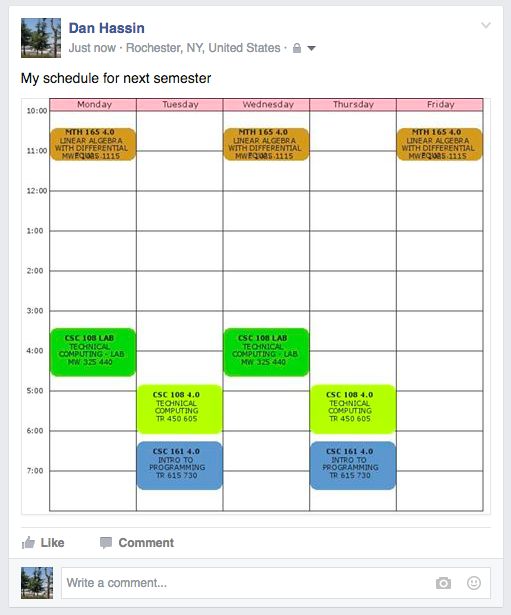
\includegraphics[width=6cm]{images/cdcs/social}
      \caption{Sharing a static schedule image generated by Better CDCS on Facebook} \label{fig:cdcs-social}
    \end{subfigure}

    \hspace{10pt}

    \begin{subfigure}[w]{7cm}
      \centering
      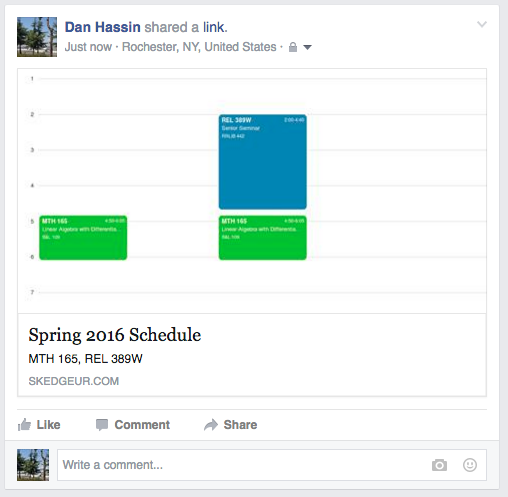
\includegraphics[width=6.1cm]{images/skedge/facebook}
      \caption{Sharing a Skedge schedule on Facebook, linked to the live and dynamic schedule share page on Skedge} \label{fig:sk-fb}
    \end{subfigure}

  \end{tabular}
  \caption{Comparison of sharing schedules on Facebook}
\end{figure}

\subsection{Limitations of the Facebook model, remedied by Skedge}

  \subsubsection{Static image vs. live site}

    As mentioned above, the schedules generated with Better CDCS cannot be shared publicly, and therefore students can only post a static image of their schedule at the time of posting. This excludes the possibility of edits to the schedule being reflected in the same post to their friends. Moreover, referencing courses (i.e. looking up more information on a course a friend is taking) is not very usable under this model as it requires a manual search.

    Skedge allows users to generate a public link (of the format \url{http://skedgeur.com/1234}, with the last four digits being a random ID for that schedule) to a view-only, larger version of their schedules (see Figure \ref{fig:sk-share}). If a user visiting others' share pages also has their schedule saved on Skedge, the option to ``overlay'' the user's schedule ontop of the share page's schedule is available, making it easier for friends to find common free time (see Figure \ref{fig:sk-overlay}).

    When this link is posted on Facebook, Skedge will include a rendered image of the schedule in the post, maintaining the element of visual bait with posting a static image (see Figure \ref{fig:sk-fb}).

    \begin{figure}[H]
      \centering
      \begin{tabular}{c c}
        \vspace{10pt}

        \begin{subfigure}[w]{10cm}
          \centering
          \fbox{
            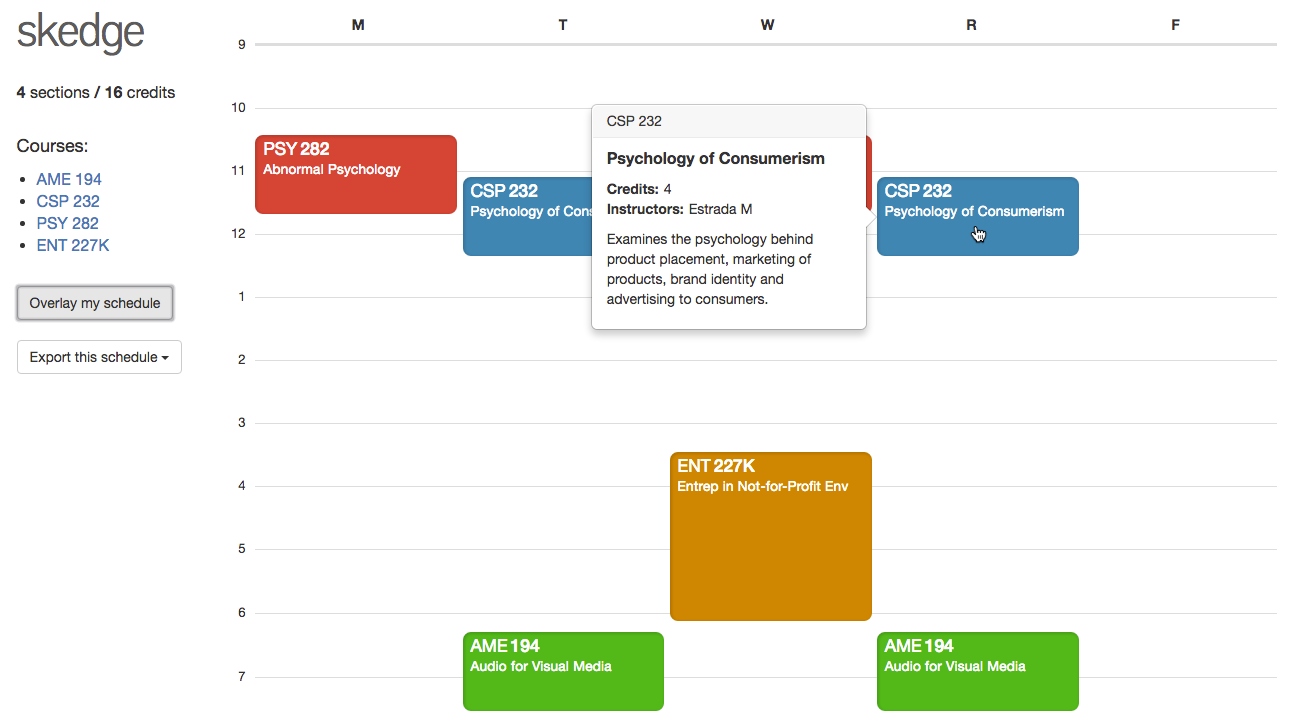
\includegraphics[width=1.00\textwidth]{images/skedge/share}
          }
          \caption{Skedge's schedule ``share'' page. Hovering over a course shows information about it, and clicking searches for it.} \label{fig:sk-share}
        \end{subfigure} \vspace{10pt}\\
        
        \begin{subfigure}[w]{10cm}
          \centering
          \fbox{
            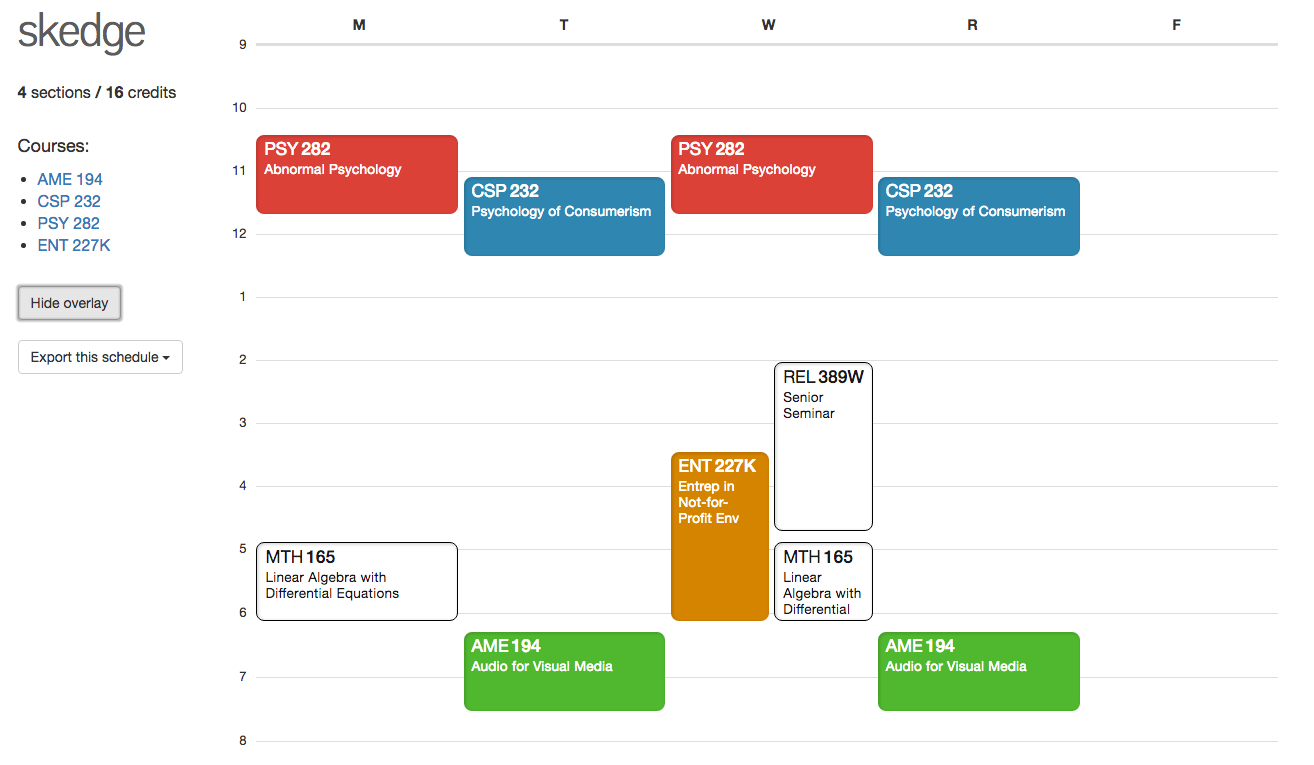
\includegraphics[width=1.00\textwidth]{images/skedge/share-compare}
          }
          \caption{The ``overlay'' feature enabled, superimposing the user's schedule over the share page's schedule.} \label{fig:sk-overlay}
        \end{subfigure}
      \end{tabular}
      \caption{Skedge's per-schedule share page}
    \end{figure}


  \subsubsection{Robustness of finding courses taken by peers}

  The Facebook model stimies users from finding courses peers are taking in several ways. It

  \begin{enumerate}
    \item requires that \textbf{a)} peers share their schedules on Facebook publicly and \textbf{b)} the user incidentally checks Facebook while that post is still deemed relevant via Facebook's algorithms.

    \item is unorganized, as schedules are spread across space and time (different posts and profiles).

    \item is only effective for the \emph{current semester}. It can be very difficult for students seeking advice (or even academic help) for a specific class to find others who had taken it before.

    \item is \emph{schedule}-oriented, not \emph{search}-oriented. Course discovery can only happen from seeing peers' schedules, not from browsing and finding classes that their peers may be taking.

  \end{enumerate}

  Solving these issues requires platform infrastructure external to Facebook, but Facebook's ubiquity is invaluable. Since Skedge already saves and archives users' schedules and Facebook has an integration API, building this platform into Skedge was the natural solution.

%figure
 
\subsection{Skedge Social}

The \emph{Skedge Social} platform aims to leverage existing social media paradigms (e.g. \emph{news feed}, \emph{likes}, and \emph{requests}) to more seamlessly give users answers to the questions alluded to earlier---``what are my friends taking?'' and ``what do my friends recommend?''. Skedge Social currently only supports Facebook, which can be integrated with a single click (see Figure \ref{fig:sk-social-login}).
  
  \begin{figure}[H]
      \centering
      \fbox{
        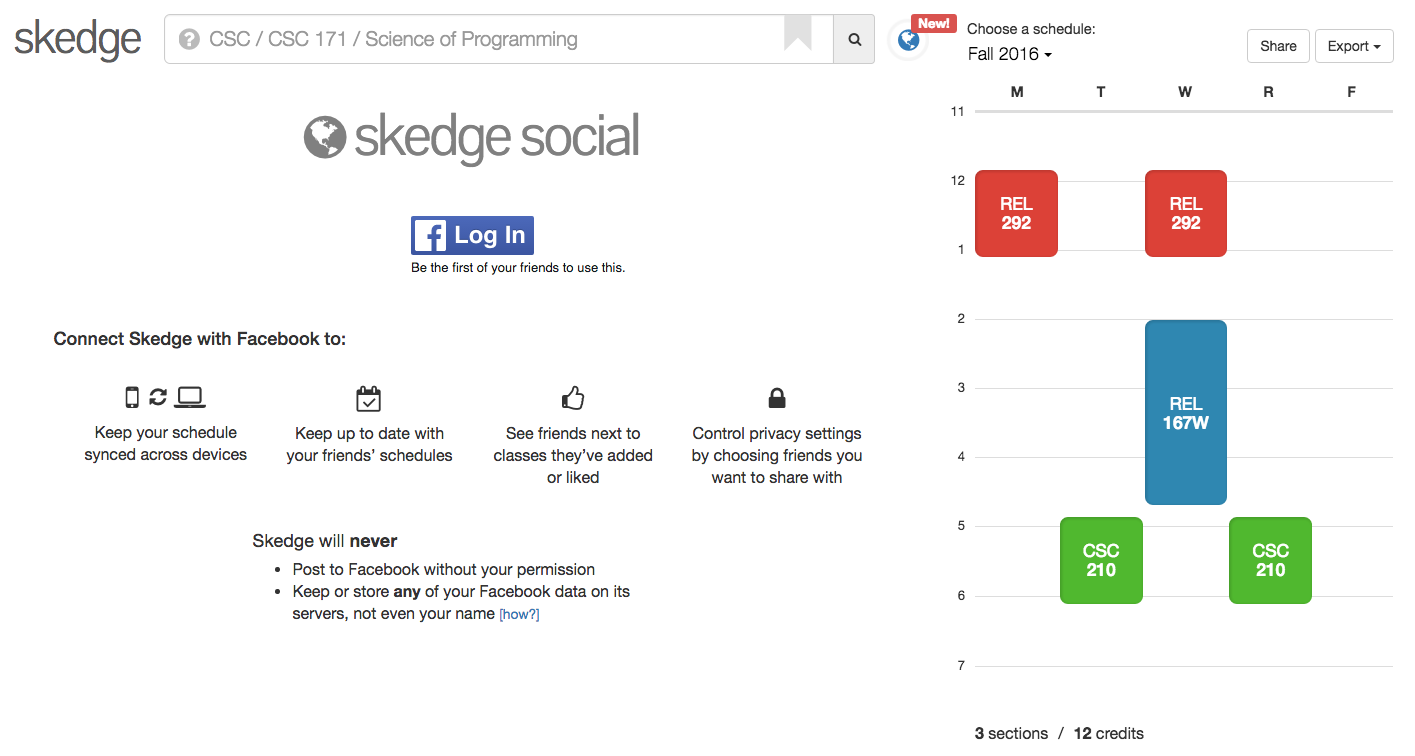
\includegraphics[width=9cm]{images/skedge/social-login}
      }
      \caption{Skedge Social landing page (\url{http://skedgeur.com/social}) for a user whose account has not yet been integrated with Facebook. Skedge Social appears in the context of the ordinary Skedge interface, and is accessible with the globe icon to the right of the searchbar.} \label{fig:sk-social-login}
    \end{figure}

  \subsubsection{Schedule feed}

  Immediately after logging in, the user will see the ``schedule feed,'' the list of the user's peers' current schedules (see Figure \ref{fig:sk-feed}). This takes from a familiar paradigm of the \emph{feed} in social networks, which is routinely scrolled for updates.[1] For each schedule, the user can visualize their own schedule side-by-side (using with the same ``overlay'' mechanic explained earlier), access the Facebook profile of the schedule's owner, and see the list of courses that user likes.

  This has the advantage of organizing and persisting peers' schedules, solving the first three issues of the ``Facebook post'' model listed above.
      
    \begin{figure}
      \centering
      \fbox{
        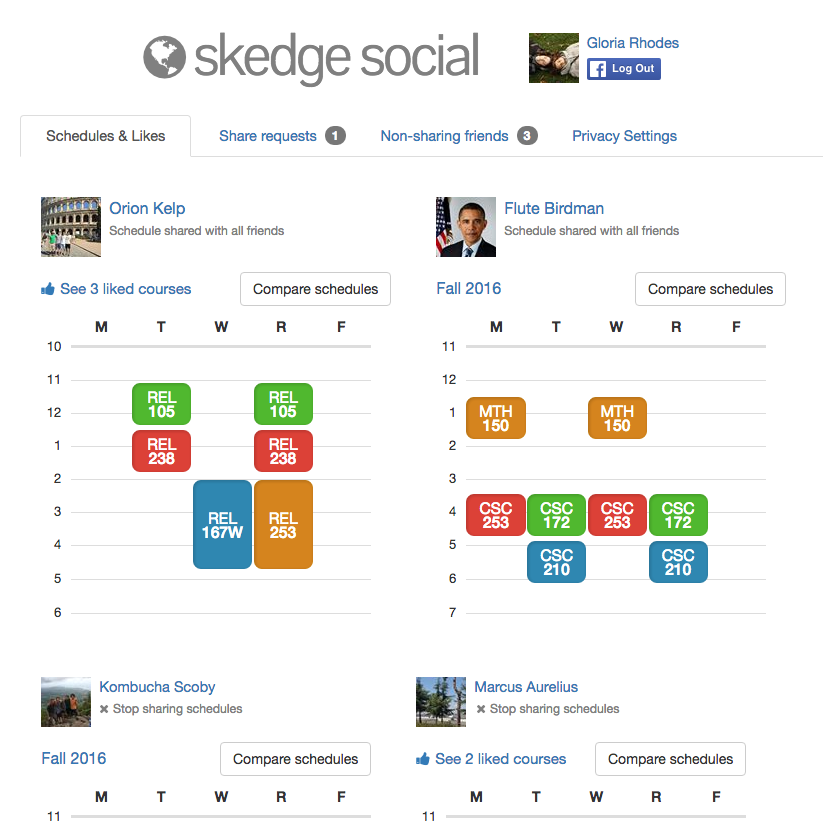
\includegraphics[width=9cm]{images/skedge/social}
      }
      \caption{Skedge Social's schedule feed (the default of four tabs) for a user who has integrated their Skedge account with Facebook. The user can toggle between a peer's schedule and the list of their \emph{liked} courses.} \label{fig:sk-feed}
    \end{figure}
  
  \subsubsection{Search result integration}

  Skedge Social also integrates into course search results, showing the user any other peers on the platform who are taking, have taken, or \emph{liked} courses in the results list (see Figure \ref{fig:sk-social-course}). This has several advantages, which solve the last ``Facebook post'' model issue listed above:

  \begin{itemize}

  \item It enhances the user's social engagement and allows them to better keep up with peers.
  \item It promotes and facilitates communication for users either seeking or soliciting advice regarding courses (sending a Facebook message is merely two clicks away).
  \item It brings attention to courses which are particularly popular or liked among the user's community of peers, increasing the chances of serendipitous course discovery.

  \end{itemize}

    \begin{figure}
      \centering
      \fbox{
        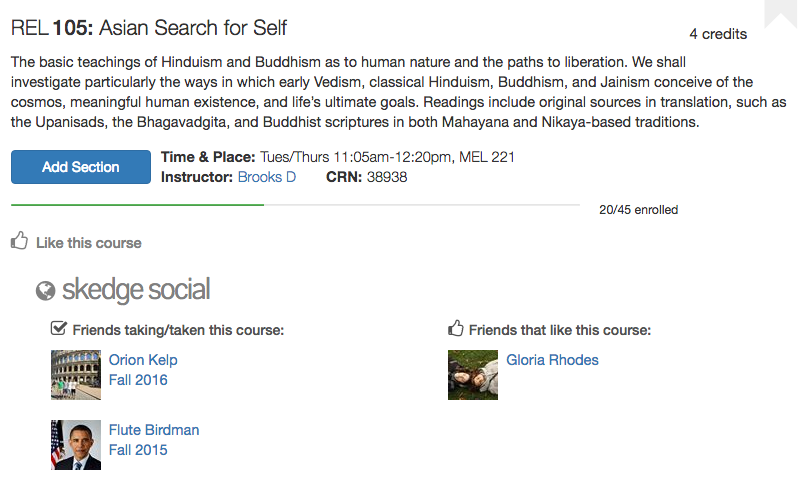
\includegraphics[width=12cm]{images/skedge/social-course}
      }
      \caption{Skedge Social integrating into a course search result} \label{fig:sk-social-course}
    \end{figure}

  \subsubsection{Personal schedule synchronization}

  For the moment, Skedge leverages a user's 

  \subsubsection{Privacy and share requests}

  Skedge offers users two privacy options:

  \begin{enumerate}
  \item ``Share my schedule and likes with all my friends'' (Public)\footnote{Note that even the ``public'' option is not truly public, as it only grants view permissions to people who are already friends with the user on Facebook.}
  \item ``Share my schedule and likes only with friends I approve'' (Private)
  \end{enumerate}

  
  

  \subsubsection{Notifications}

  \begin{figure}[H]
    \centering
    \begin{tabular}{c c}
      \begin{subfigure}[w]{3cm}
        \centering
        
\includegraphics[height=1.5cm]{images/skedge/social-note1}
        \caption{Note1.} \label{fig:sk-social-note1}
      \end{subfigure}
      
      \begin{subfigure}[w]{3cm}
        \centering
        
\includegraphics[height=1.5cm]{images/skedge/social-note2}
        \caption{Note2.} \label{fig:sk-social-note2}
      \end{subfigure}
    \end{tabular}
    \caption{Notifications}
  \end{figure}

